\documentclass[10pt, a4paper]{article}
\usepackage{times}
\usepackage{titlesec}
\usepackage{graphicx}
\usepackage{lipsum}

\titlespacing*{\section}
{15pt}{0.75\baselineskip}{.55\baselineskip}
\titlespacing*{\subsection}
{12pt}{.5\baselineskip}{.25\baselineskip}
\titlespacing*{\subsubsection}
{11pt}{.3\baselineskip}{.1\baselineskip}
\title{Projeto POO\\
        Simulação de Casas Inteligentes}
\author{Bruno Gião a96544 \\ Miguel Vaz a72161 \\ João Cruz a95375 \\ Grupo 1}
\date{UM, LCC, 2021/2022}

\begin{document}
\maketitle

\newpage
\tableofcontents
\newpage

\section{Introdução}
\lipsum[1]
\section{Classes Base}
\lipsum[1]
\subsection{SmartDevices}
\lipsum[1]
\subsection{SmartHouse}
\lipsum[1]
\subsection{Fornecedor de Energia}
\lipsum[1]
\section{Simulador}
\lipsum[1]
\subsection{MVC}
\lipsum[1]
\subsubsection{Visualizador}
\lipsum[1]
\subsubsection{Modelo}
\lipsum[2]
\subsubsection{Controlador}
\lipsum[2]
\section{Diagrama UML}
Segue, a seguir o diagrama UML deste projeto:
\begin{figure}
        \centering
        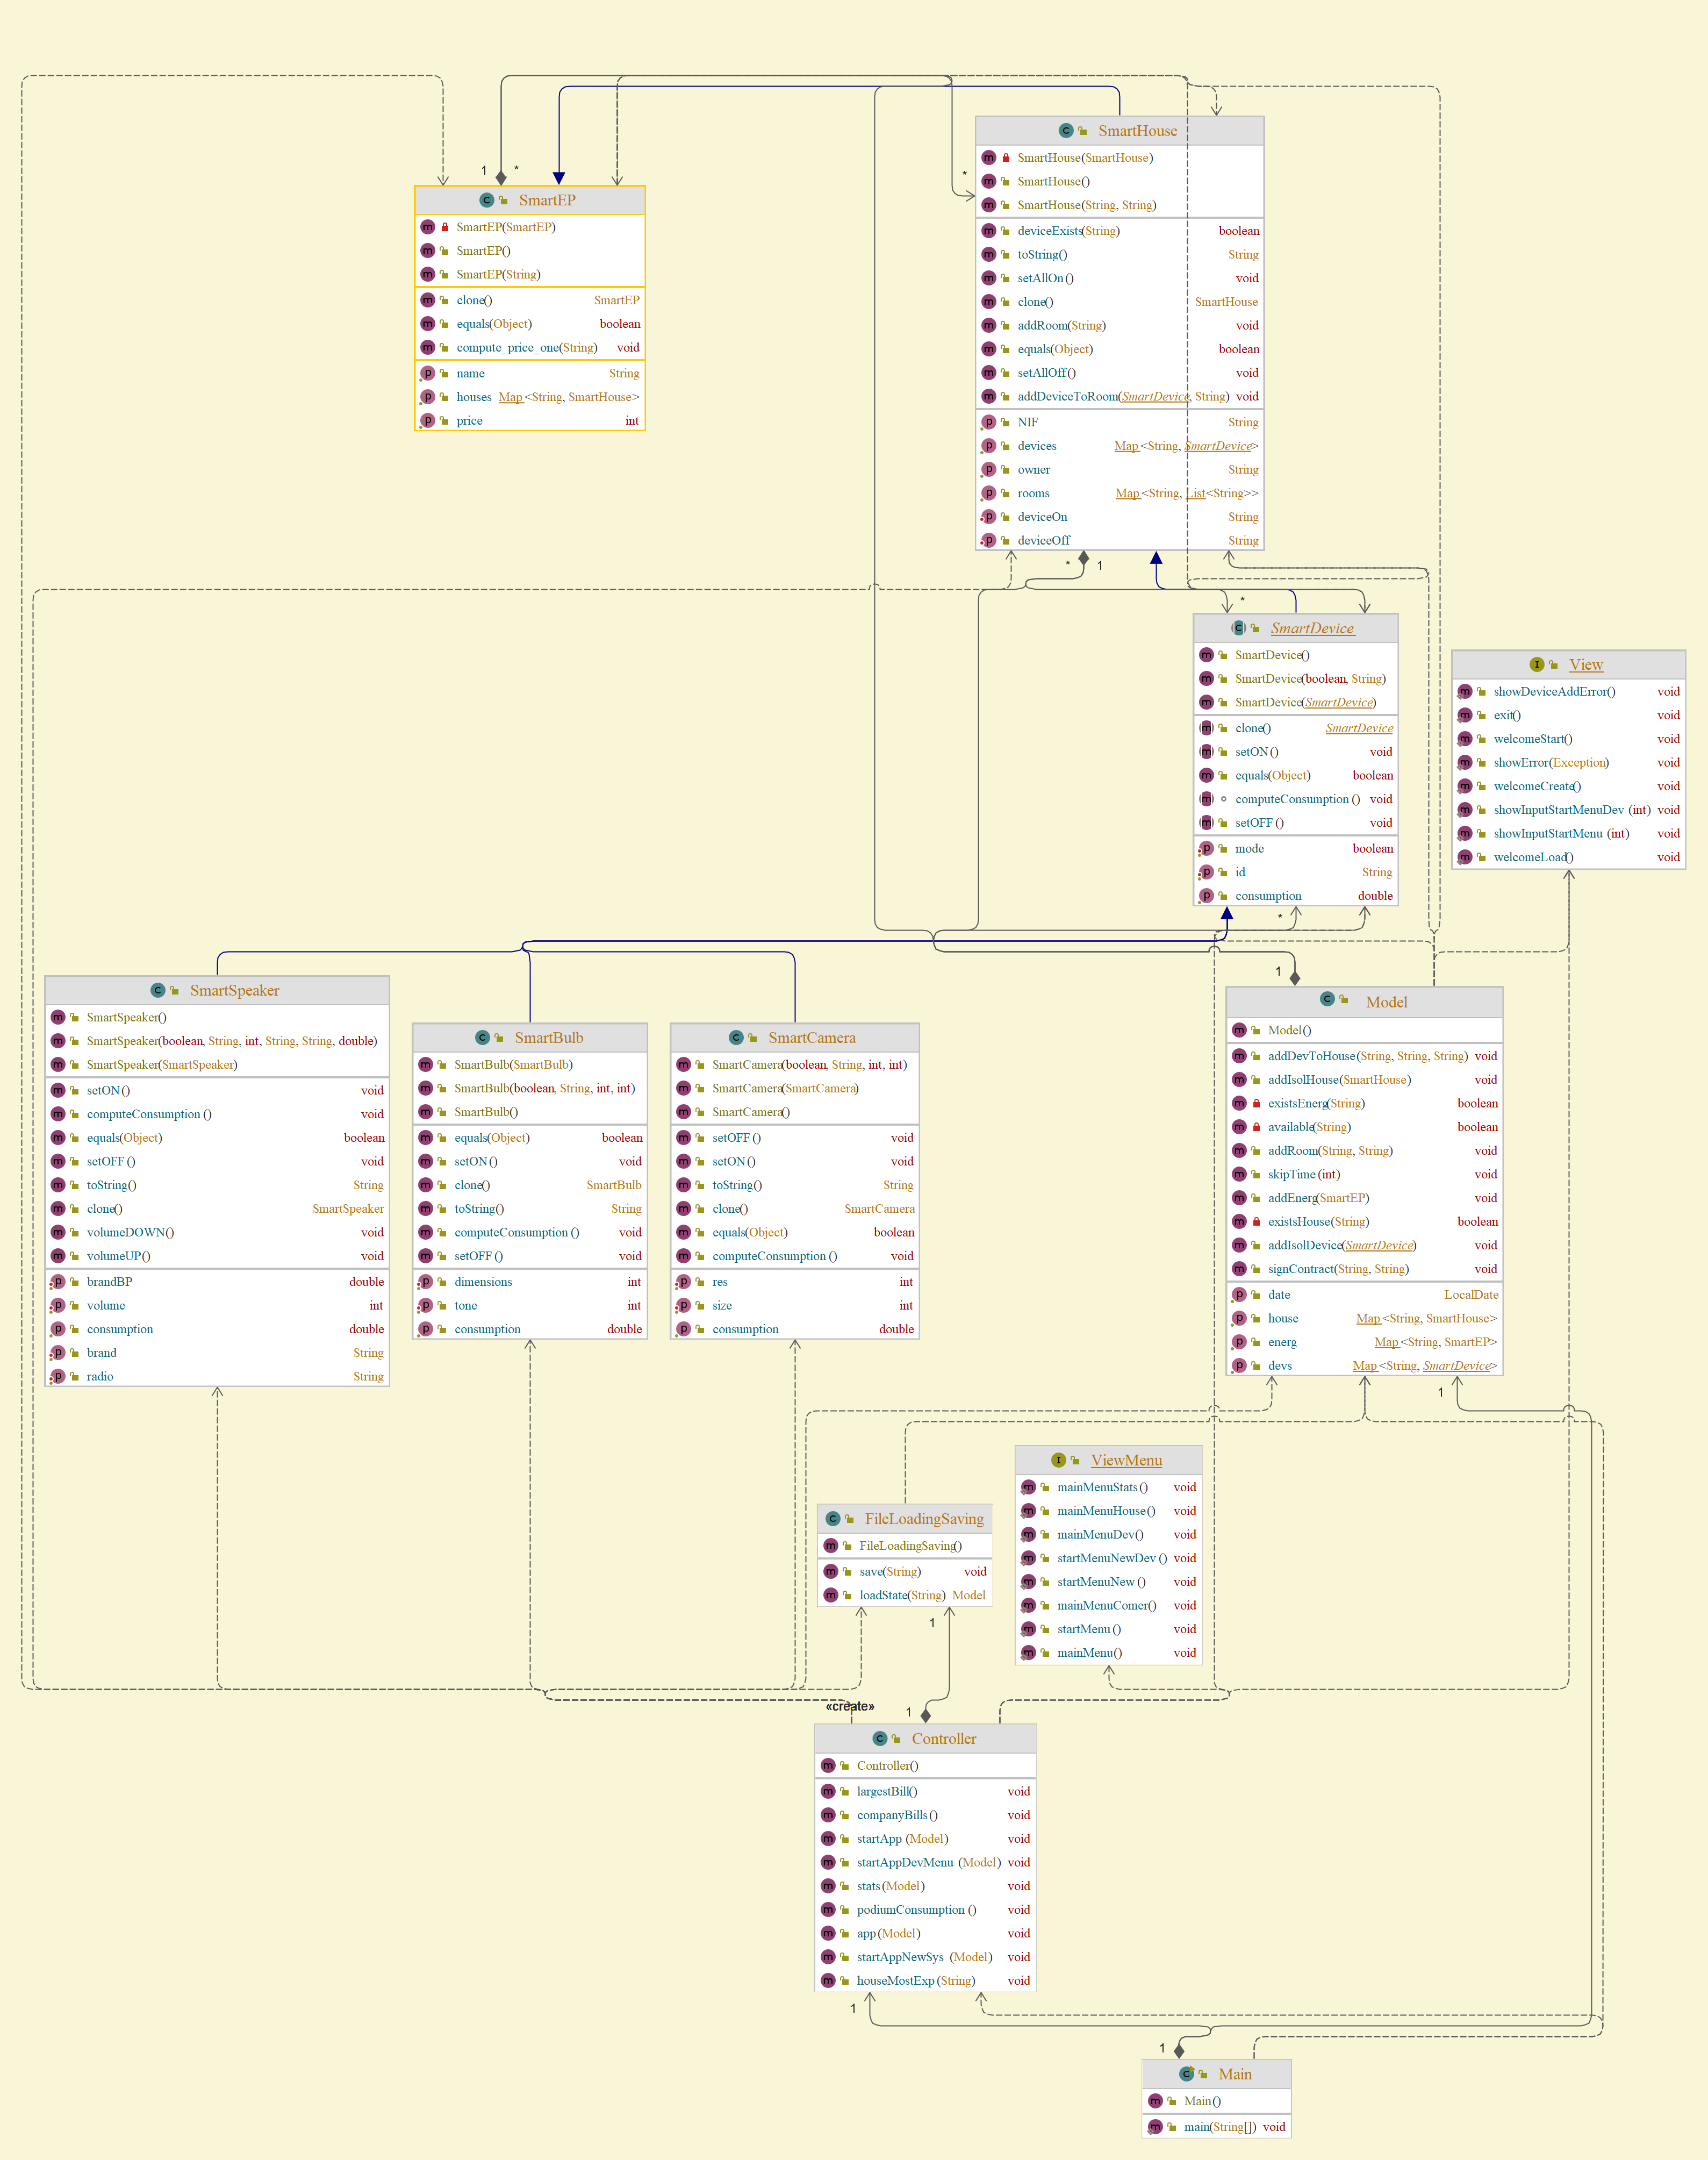
\includegraphics[width=\textwidth]{diagram.png}
\end{figure}

\newpage
\section{Conclusão}
\lipsum[1-2]
\end{document}
